\documentclass[11pt]{amsart}
\usepackage[utf8]{inputenc}
\usepackage[a4paper, total={6in,8in}, portrait, margin=0.7in]{geometry}
\usepackage{amssymb}

%Add any packages you need here
\usepackage{graphicx}
\usepackage{amsmath}
\usepackage{amsfonts}
\usepackage{float}
\usepackage{natbib}
\usepackage{listings}
\usepackage[misc]{ifsym}
\usepackage{indentfirst} 
\usepackage{amsthm}
\usepackage{appendix}

%Any functions you wanna define, pop 'em here
\newtheorem{theorem}{Theorem}[section]
\newtheorem{remark}[theorem]{Remark}
\newtheorem{definition}[theorem]{Definition}
\newtheorem{example}[theorem]{Example}
\newtheorem{lemma}[theorem]{Lemma}

\title{Improving Duckworth-Lewis: Statistical Methods for Revising Score Targets in Limited Overs Cricket}
\author{Matthew Knowles}
\date{Autumn Term 2021}

\begin{document}

\maketitle

\section{Introduction and Aims}
In recent years, the use of data science in sport has become far more common place. In cricket in particular, questions are asked about metrics such 
as run-rates or bowling economy (average of how many runs conceeded for every ball bowled) in order to select a starting XI with the best lineup. 
Data can give a great insight into a team's performance, and if used correctly can aid a team greatly in their performance in competitions.  The vast amount
of data available is also helpful in finding patterns in matches. This is the area of focus for this project. \\

The specific aim of this project is to use more sophisticated methods for revising score targets in limited overs cricket. For the reader unfarmiliar 
with the game of cricket. Two teams have 50 'overs' each to score as many 'runs' as possible. However, sometimes, a rain delay, pitch invasion 
or other interruption leaves the team batting second with less time to complete their overs. For this reason, Duckworth and Lewis, two British 
statisticians wrote a paper outlining a method for how score targets are reset given the state of play when the interruption happened. \citep{duckworth} \\

We begin by looking at the maths behind the Duckworth-Lewis method, and the extension made by Stern (REF) in the early 2000s. We look at problems
with this method, and how it is vulnerable to certain biases. Further, an investigation is undertaken into a few statistical methods aimed to 
reduce the exposure of the method to certain biases, the main method we look at here uses techniques from Bayesian Statistcs (REF).\\

Following on from this, we undertake some exploratory data analysis to look for immediate patterns in the match data we have, and to influence decisions
that need to be made in building the models that are the central aspect of the project. 

\section{Data}
\subsection{Data Origin}
The primary source of data for carrying out this project was downloaded from ``cricsheet''\footnote{https://cricsheet.org/}
and stored locally on a private server. In total there are 2167 individual matches of data. Each in a JSON format.
These cover matches ranging from the $3^{rd}$ of January, 2004. Up to the $20^{th}$ of July, 2021.

\subsection{Attributes}
Each JSON file contains a considerable amount of metadata surrounding the match in question. Along with 
ball-by-ball data for the entire match. We have access to attributes such as the date, where the match was played,
the entire teamsheet for both teams, who the officials were, who won- and by what margin, who won the toss; and many others.

We also have the ball-by-ball data. So for every ball bowled, it gives who were the striking and non-striking batsmen, how many runs
were scored and how. It also details if a wicket was taken that ball, and how.

\subsection{Pre-Processing}
In order to get data in to a usable form, Python scripts were written to read the JSON files and extract features necessary for this project.
These Python scripts output CSV files that can be fed into R for easier statistical analysis. For example, when training the neural network model,
a Python script was built to extract the runs scored in each over for over 1400 games. The labelled CSV data was then used by an R script to 
output a matrix of runrates and corresponding final runs, which was used to train the Neural Network.

\subsection{Problems with the Data}
When it comes to machine learning, the more data the better is a general rule. Now this can sometimes lead to sub-problems, such as overfitting. But on the whole.
it is much better to have as much data as possible. We will be training a neural network on 1435 data points. Stictly speaking, this isn't a lot of data, but there
isn't much that can be done about this due to the cricketing calender only having a certain number of limited-overs matches each year.

\section{Duckworth-Lewis}
We begin by looking at the main equation that is the backbone of the Duckworth-Lewis method.

\begin{equation}
    \label{dleq}
    Z(u,w) = Z_0(w)[1-exp(-b(w)u)]
\end{equation}

In \ref{dleq}, u represents the number of overs the runs are scored in, w is the number of wickets lost, and b(w) is an exponential decay constant.
Due to commercial reasons, the authors were unble to publish some of the mathematical constants that they used. For that reason, we create a plot of this relationship
using several rough values based on knowledge of the game. although not perfect, it still gives an idea for how this relationship behaves, which is the important thing.

\begin{figure}
    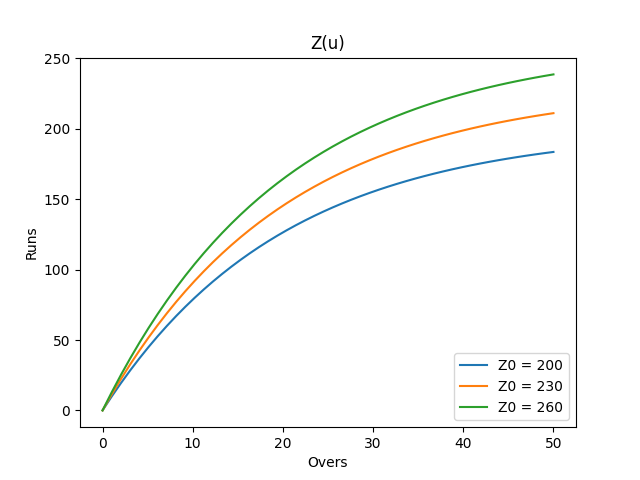
\includegraphics[scale=0.6]{../Thesis/figures/z(u).png}
\end{figure}

We can see how the runs scored drops off towards the end of the innings. 

\section{Neural Networks}
At the time of writing, the Neural Network is still under construction.

\bibliography{../Thesis/refs}{}
\bibliographystyle{plain}

\end{document}